\documentclass[12pt]{article}
\usepackage{amsmath, amssymb}
\usepackage{booktabs}
\usepackage{geometry}
\usepackage{xcolor}
\usepackage{hyperref}
\usepackage{array}
\usepackage{graphicx}
\usepackage{caption}
\usepackage{longtable}
\usepackage{multirow}
\geometry{margin=1in}

\definecolor{noteblue}{RGB}{0,70,160}
\definecolor{actiongreen}{RGB}{0,120,0}
\newcommand{\note}[1]{{\color{noteblue}\textit{#1}}}
\newcommand{\action}[1]{{\color{actiongreen}#1}}

\title{$\gamma_{\text{PrEP}}$ Payer-Mix Sensitivity Analysis:\\[2pt]
       \large Meeting Follow-Up and Revised-Parameter Results}
\date{August 13, 2026}

\begin{document}
\maketitle

\begin{abstract}
\noindent
Part~I of this memo reproduces the August 10, 2026 meeting follow-up
(\texttt{INFORM-HIV-Analysis/Raff\_tmp/gamma\_prep\_meeting\_followup.tex}),
which identified that the model's PrEP private-insurance-floor parameter
($r = 0.78$, national) is likely too high for INFORM-HIV's population
(young Black MSM/TGW in Chicago) and proposed a working value of
$r \approx 25\%$. Part~II presents the results of actually running that
revised value through the cost-mapping pipeline: a point-estimate
comparison against the current committed baseline, and a small Monte Carlo
sensitivity sweep over $r$ and the baseline PrEP coverage anchor $P^0$.
\end{abstract}
\tableofcontents
\bigskip

\part{Meeting Follow-Up (2026-08-10)}
\label{part:meeting}

%% =========================================================================
\section{Jonathan's question: why is it $P - \gamma$, not $P \times \gamma$?}
\label{sec:equation}

The coverage model (main text, Eqs.~1--2) is:
\begin{align}
P_{\text{ART}}  &= \min\!\left(1,\; \frac{G_{\text{ART}}}{\alpha\, C_{\text{ART}}\, N_{\text{HIV+}}} + \gamma_{\text{ART}}\right), \label{eq:PART} \\[4pt]
P_{\text{PrEP}} &= \min\!\left(1,\; \frac{G_{\text{PrEP}}}{\beta\, C_{\text{PrEP}}\, N_{\text{HIV-}}} + \gamma_{\text{PrEP}}\right). \label{eq:PPrEP}
\end{align}

Jonathan's question concerned the calibration equations (supplement, Eqs.~4--5),
which solve for $\alpha$ and $\beta$ given an observed baseline coverage
$P^{0}$:
\begin{align}
\alpha &= \frac{G_{\text{ART}}}{(P_{\text{ART}}^{0} - \gamma_{\text{ART}})\, C_{\text{ART}}\, N_{\text{HIV+}}}, \label{eq:alpha_cal} \\[4pt]
\beta  &= \frac{G_{\text{PrEP}}}{(P_{\text{PrEP}}^{0} - \gamma_{\text{PrEP}})\, C_{\text{PrEP}}\, N_{\text{HIV-}}}. \label{eq:beta_cal}
\end{align}
Why $(P^{0} - \gamma)$ and not $(P^{0}\times \gamma)$?

\subsection{The subtraction is algebra, not a separate modeling choice}

Equations~\eqref{eq:alpha_cal}--\eqref{eq:beta_cal} are not an independent
assumption. They are what you get by taking the \emph{forward} model,
Eqs.~\eqref{eq:PART}--\eqref{eq:PPrEP}, and solving for $\alpha$ (or $\beta$)
at the observed baseline. Concretely, for ART:
\[
P_{\text{ART}}^{0} = \frac{G_{\text{ART}}}{\alpha\, C_{\text{ART}}\, N_{\text{HIV+}}} + \gamma_{\text{ART}}
\]
\[
\quad\Longrightarrow\quad
\underbrace{P_{\text{ART}}^{0} - \gamma_{\text{ART}}}_{\text{government-attributable share}}
= \frac{G_{\text{ART}}}{\alpha\, C_{\text{ART}}\, N_{\text{HIV+}}}
\]
\[
\quad\Longrightarrow\quad
\alpha = \frac{G_{\text{ART}}}{(P_{\text{ART}}^{0} - \gamma_{\text{ART}})\, C_{\text{ART}}\, N_{\text{HIV+}}}.
\]
The subtraction appears because the forward model is \textbf{additive}:
total coverage is a private floor $\gamma$ (assumed fixed, unaffected by
government spending) \emph{plus} a government-driven increment
$G/(\alpha C N)$, capped at~1. Isolating ``how much of the observed coverage
is attributable to government spending'' is therefore just $P^{0}$ minus the
part we've already assumed is privately financed --- a subtraction, by
construction.

\subsection{The modeling choice that actually matters}

The real assumption is one level up: coverage is additive
(private floor + government increment), not multiplicative (e.g., government
funding scaling up access among the population \emph{not} already privately
covered, or some other interaction form). We chose the additive form for
parsimony; its limitations (nonlinearity, insurance-stratum heterogeneity,
threshold effects) are flagged in the main text as directions for future
refinement.

\subsection{Why this means $\alpha,\beta$ are not free parameters}

A direct consequence, and the reason this matters for the meeting's
discussion: once $\gamma$ and the observed baseline $P^{0}$ are fixed,
$\alpha$ (or $\beta$) is \emph{determined} by
Eq.~\eqref{eq:alpha_cal}/\eqref{eq:beta_cal} --- it is not independently
chosen or estimated. This means we \textbf{cannot revise
$\gamma_{\text{PrEP}}$ in isolation}: any change to $\gamma_{\text{PrEP}}$
requires recalibrating $\beta$ in the same step, or the model will no
longer reproduce the observed baseline PrEP coverage.

\subsection{A useful analytical fact: what actually drives cut-sensitivity}

It's worth separating two questions:

\begin{itemize}
  \item \textbf{Question 1 (coverage level):} what is $P^{0}_{\text{PrEP,obs}}$
    for young Black MSM/TGW in Chicago? (Current model: 36\%, national.
    Evidence suggests 20--24\% may be more appropriate for this population.)
  \item \textbf{Question 2 (payer mix):} what fraction $r$ of PrEP users in
    this population have private/non-public coverage that would survive a
    government funding cut? (Current model: $r = 0.78$, national, giving
    $\gamma_{\text{PrEP}} = r \times P^{0} = 0.78 \times 0.36 \approx 0.28$.)
\end{itemize}

Define the \emph{pass-through fraction} --- the share of observed baseline
coverage that would be lost under a 100\% funding cut (i.e., $\Delta=1$,
so $P \to \gamma$):
\[
\text{pass-through} = \frac{P^{0} - \gamma}{P^{0}} = \frac{P^{0} - r P^{0}}{P^{0}} = 1 - r.
\]
For PrEP, $1 - 0.78 = 22\%$; for ART, $1 - \gamma_{\text{ART}}/P^{0}_{\text{ART}} =
1 - 0.15/0.62 \approx 76\%$.

\note{The important implication: the \emph{relative} pass-through fraction
depends only on $r$ (Question 2), not on $P^{0}$ (Question 1), because
$\gamma = r P^{0}$ by construction, so $P^0$ cancels out of the ratio. If we
only revise the coverage-level anchor (36\%~$\to$~24\%) while keeping the
national $r=0.78$, the model's relative sensitivity to funding cuts is
\emph{unchanged} (still $\sim$22\% pass-through). Only the absolute number
of percentage points at risk would shrink. Part~II of this memo verifies
this claim numerically.}

%% =========================================================================
\section{Summary of the 2026-08-10 meeting}
\label{sec:summary}

\subsection{The problem, restated}

\begin{itemize}
  \item $\gamma_{\text{PrEP}} = 0.28$ was derived entirely from national data:
    a national baseline PrEP coverage of 36\% (CDC Monitoring 2022) and a
    national payer-mix estimate that 78\% of PrEP users are privately insured
    (CDC NHBS 2024 / Bonacci et al.\ 2023).
  \item INFORM-HIV simulates a specific population --- young Black MSM/TGW in
    Chicago --- for whom both numbers are likely wrong in the same direction:
    NHBS puts Black MSM PrEP use at $\sim$24\% nationally (vs.\ 57\% for White
    MSM), and Black MSM are known to rely far more on Medicaid/Ryan
    White/ADAP and less on private insurance than PrEP users nationally.
  \item If $r=0.78$ is too high for this population, the model currently
    overstates how much PrEP access survives a funding cut, and therefore
    \emph{understates} the harm of PrEP funding cuts specifically for the
    population the paper is about.
\end{itemize}

\subsection{What we checked, and what we found}

\begin{itemize}
  \item \textbf{John Peller's (AFC) email}, forwarded by Anna, estimates
    32--33\% of Illinois residents are covered by ERISA-governed
    self-insured employer plans, 23--25\% by state-regulated fully insured
    plans, 35--36\% by public programs, and 6--7\% are uninsured. This
    addresses a different policy channel (removal of the USPSTF Grade~A
    PrEP mandate) rather than the government-funding-reduction channel our
    model represents, but is a useful sanity-check bound: combined
    commercial coverage state-wide is only $\sim$55--58\%, well below the
    78\% assumed among PrEP users --- consistent with, but not proof of,
    $r=0.78$ being too high for a lower-income, more publicly-insured
    subpopulation.
  \item A targeted literature search (AIDSVu/PrEPVu.org, CDC MMWR 2019
    23-urban-areas NHBS report, the AJPH 2021 Medicaid-expansion NHBS study
    covering 22 cities including Chicago, and a 2018--2022 pharmacoequity
    claims analysis) confirmed that \textbf{no published source crosses
    race/ethnicity with PrEP-payer type}. This looks like a genuine gap in
    the literature.
  \item The Black--white PrEP-use gap persists \emph{even among the
    insured}, and the AJPH study found the racial gap persists regardless
    of Medicaid-expansion status --- insurance/payer source is not the
    whole story; a revised $r$ corrects the financing piece but should not
    be read as fully correcting for the underlying access disparity.
  \item Meg McElroy's ADAP FOIA summary (Illinois-specific, uninsured vs.\
    insured client counts, April 2024--March 2025) could serve as a
    partial cross-check, though it is not stratified by race.
\end{itemize}

\subsection{Where the discussion landed}

We agreed to set $r \approx 25\%$ as a working value:
\begin{itemize}
  \item this is a \textbf{post-hoc recalculation} --- it only touches the
    funding-to-coverage layer, not the underlying ABM, so no new simulation
    is required;
  \item $\beta$ must be recalibrated alongside any revision to
    $\gamma_{\text{PrEP}}$ (Section~\ref{sec:equation});
  \item getting an expert read from AFC (John Peller/Meg McElroy) on a
    defensible number would be more credible than an internal guess.
\end{itemize}

%% =========================================================================
\section{Action plan (from the 2026-08-10 meeting)}
\label{sec:action}

\action{\begin{enumerate}
  \item Settle on a working value/range for $r$ (equivalently, $\gamma_{\text{PrEP}}$).
  \item Recalibrate $\beta$ (and audit $\gamma_{\text{ART}}/\alpha$ the same
    way) using Eqs.~\eqref{eq:alpha_cal}--\eqref{eq:beta_cal}.
  \item Send AFC a narrower, specific data request: among PrEP users who are
    young Black MSM/TGW in Chicago, what fraction access PrEP via private
    insurance vs.\ Medicaid/ADAP/PrEP4Illinois/uninsured?
  \item \textbf{Re-run the cost-mapping layer with the revised parameters}
    --- regenerating the forest plot, the ribbon+heatmap panel, and the
    scenario table --- and mirror the same parameter change in
    \texttt{INFORM-HIV-App}.
  \item Document the limitation explicitly in the supplementary appendix: a
    race/city-stratified PrEP payer-mix estimate does not appear to exist in
    the published literature.
\end{enumerate}}

Part~II below carries out item 4 above as an exploratory sensitivity check
(not yet the paper's committed figures --- see Section~\ref{sec:status}).

%% =========================================================================
\part{Sensitivity Analysis Results (2026-08-13)}
\label{part:results}

\section{What was run}
\label{sec:methods}

Using \texttt{04\_cost\_mapping/sensitivity/} (branch
\texttt{sensitivity/gamma-prep-r-p0} of
\texttt{INFORM-HIV-Funding-Scenario-Exploration}), we recalibrated
$\gamma_{\text{PrEP}}$ and $\beta_{\text{PrEP}}$ from a chosen $(r, P^0)$
pair via Eqs.~\eqref{eq:alpha_cal}--\eqref{eq:beta_cal}
(\texttt{R/recalibrate.R}), then queried the same stage-03 incidence
surrogate and common-random-numbers machinery
(\texttt{compute\_scenario\_draws\_crn()}) the main-text forest plot uses,
without rebuilding the full $101\times101$ grid. Three parameter sets:

\begin{itemize}
  \item \textbf{Baseline} --- current committed values: $r=0.78$,
    $P^0 \approx 36\%$ (i.e.\ $\gamma_{\text{PrEP}}=0.28$, $\beta_{\text{PrEP}}=4.0$).
  \item \textbf{Case 1} --- $r=25\%$, $P^0$ unchanged ($\approx 36\%$).
  \item \textbf{Case 2} --- $r=25\%$, $P^0=24\%$ (both the payer-mix and the
    baseline-coverage-level anchor revised).
\end{itemize}

Two important scope notes: (1) this uses only the pure-computation modules
(\texttt{parameters.R}, \texttt{irr\_common\_random\_numbers.R}) and plain
\texttt{ggplot2} output --- it does \textbf{not} use
\texttt{plot\_forest.R}/\texttt{plot\_ribbon.R}, which require the RAND
house-style package \texttt{randplot} that is not currently installed and
will need to be requested from Pedro before the paper's actual figures can
be regenerated with the revised parameter. (2) Nothing in
\texttt{cost\_params.yml} or the tracked \texttt{output/} directory on
\texttt{main} was touched --- the paper's currently committed $r=0.78$
baseline is unchanged.

\section{Case comparison: current vs.\ revised $r$}
\label{sec:case-comparison}

Table~\ref{tab:case-comparison} reports the mean incidence rate ratio (IRR,
year-10, vs.\ the no-cut baseline) with 95\% credible intervals, for three
government-funding-reduction scenarios at 10/25/40\% cuts. \textbf{Case~1
and Case~2 are numerically identical} on every row (verified to
floating-point precision by construction, not just approximately) ---
directly confirming the analytical claim in Section~\ref{sec:equation}:
$(P^0-\gamma_{\text{PrEP}})/P^0 = 1-r$ is algebraically independent of
$P^0$. Only $r$ is shown in the table below as a result.

\begin{table}[htbp]
\centering
\caption{Mean incidence rate ratio (95\% CI) by scenario and funding-reduction level.}
\label{tab:case-comparison}
\begin{tabular}{llcc}
\toprule
Scenario & Funding cut & Current ($r=0.78$) & Revised ($r=25\%$) \\
\midrule
\multirow{3}{*}{Reduce PrEP only}
  & 10\% & 1.009 [0.998, 1.020] & 1.033 [1.000, 1.065] \\
  & 25\% & 1.024 [0.998, 1.049] & 1.085 [1.017, 1.159] \\
  & 40\% & 1.039 [1.001, 1.076] & 1.135 [1.043, 1.235] \\
\addlinespace
\multirow{3}{*}{Reduce ART only}
  & 10\% & 1.139 [1.108, 1.171] & 1.139 [1.108, 1.171] \\
  & 25\% & 1.367 [1.304, 1.425] & 1.367 [1.304, 1.425] \\
  & 40\% & 1.588 [1.498, 1.684] & 1.588 [1.498, 1.684] \\
\addlinespace
\multirow{3}{*}{Reduce both PrEP and ART}
  & 10\% & 1.149 [1.119, 1.179] & 1.176 [1.135, 1.215] \\
  & 25\% & 1.399 [1.338, 1.459] & 1.474 [1.384, 1.573] \\
  & 40\% & 1.645 [1.558, 1.759] & 1.775 [1.644, 1.943] \\
\bottomrule
\end{tabular}
\end{table}

The ART-only rows are identical between columns by construction (the ART
payer-mix parameter $\gamma_{\text{ART}}$ was not touched); the PrEP-only
and combined rows show a consistently larger incidence-rate-ratio under the
revised, lower $r$ --- the effect widens as the funding cut deepens.

\begin{figure}[htbp]
\centering
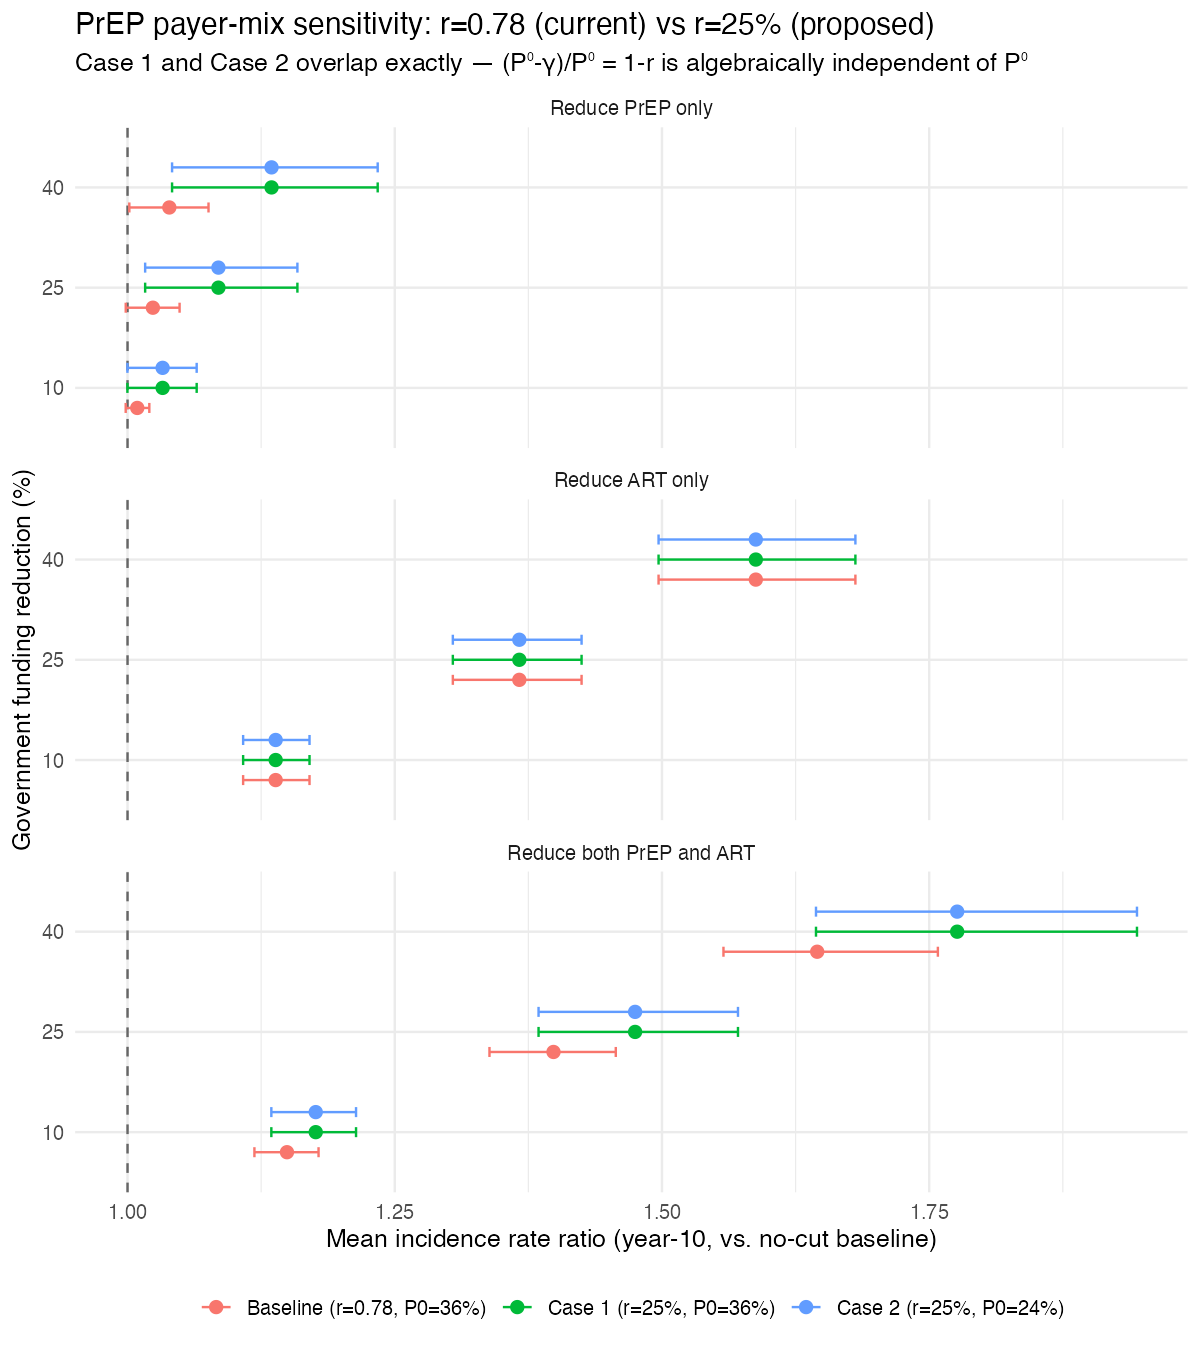
\includegraphics[width=0.85\textwidth]{figures/case_comparison_forest.png}
\caption{Forest-style comparison of mean incidence rate ratio across the
three funding-cut scenarios, current ($r=0.78$) vs.\ revised ($r=25\%$,
both $P^0$ variants). Case~1 and Case~2 overlap exactly.}
\label{fig:forest}
\end{figure}

\begin{figure}[htbp]
\centering
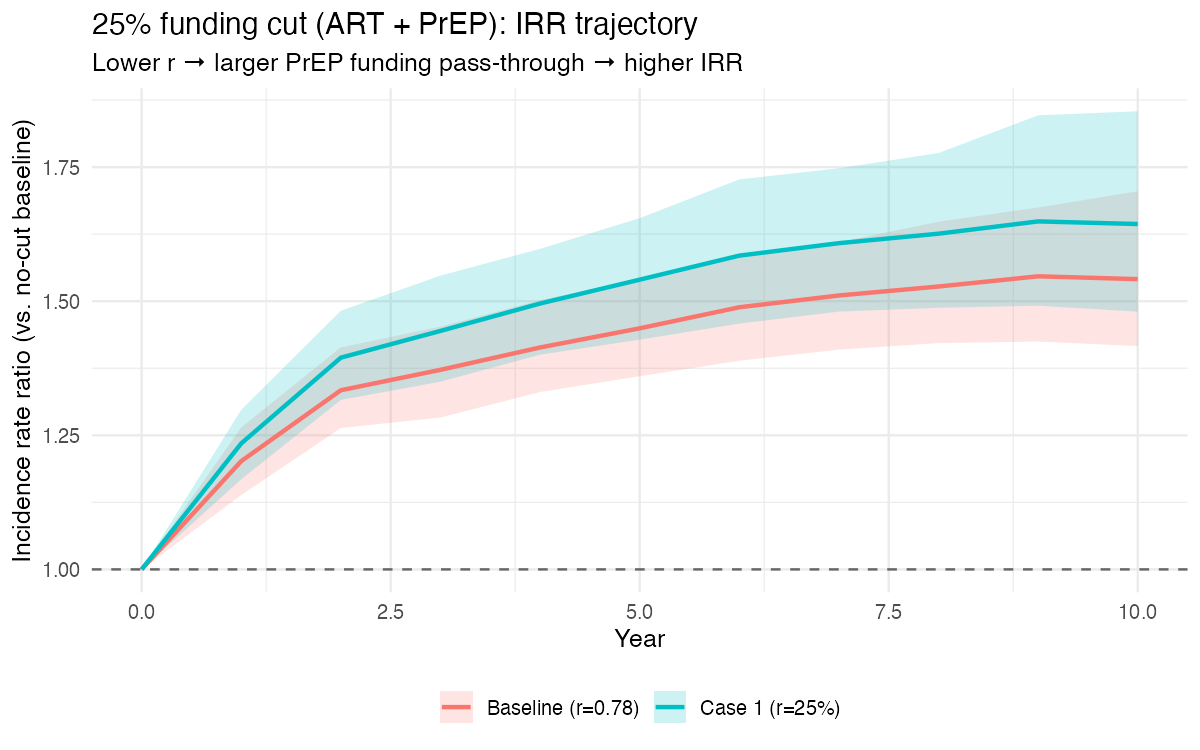
\includegraphics[width=0.75\textwidth]{figures/trajectory_comparison.png}
\caption{Year-by-year incidence-rate-ratio trajectory for a 25\% government
funding cut applied to both ART and PrEP simultaneously, current vs.\
revised $r$.}
\label{fig:trajectory}
\end{figure}

\section{Monte Carlo sensitivity to $r$ and $P^0$}
\label{sec:mc}

To check how sensitive the headline result is to uncertainty in the
revised parameters themselves, we drew $N=200$ independent joint samples of
$r \sim \text{Uniform}(0.125, 0.375)$ and $P^0 \sim
\text{Uniform}(0.12, 0.36)$ (each $\pm 50\%$ around the Case~2 mode,
$r=25\%$/$P^0=24\%$), recalibrated $\gamma_{\text{PrEP}}/\beta_{\text{PrEP}}$
for each draw, and queried the single headline scenario (25\% government
funding cut, both ART and PrEP) for each.

\begin{itemize}
  \item IRR ranged from 1.457 to 1.491 across the 200 draws (mean 1.474).
  \item $\text{cor}(\text{IRR}, r) = -1.000$ --- an almost perfectly linear
    relationship; lower $r$ (more Medicaid/ADAP-reliant payer mix) means a
    larger funding pass-through and a higher incidence rate ratio.
  \item $\text{cor}(\text{IRR}, P^0) = -0.016$ --- statistically and
    practically zero, the empirical confirmation of the algebraic claim
    that $P^0$ does not affect the incidence/IRR outcomes.
\end{itemize}

\begin{figure}[htbp]
\centering
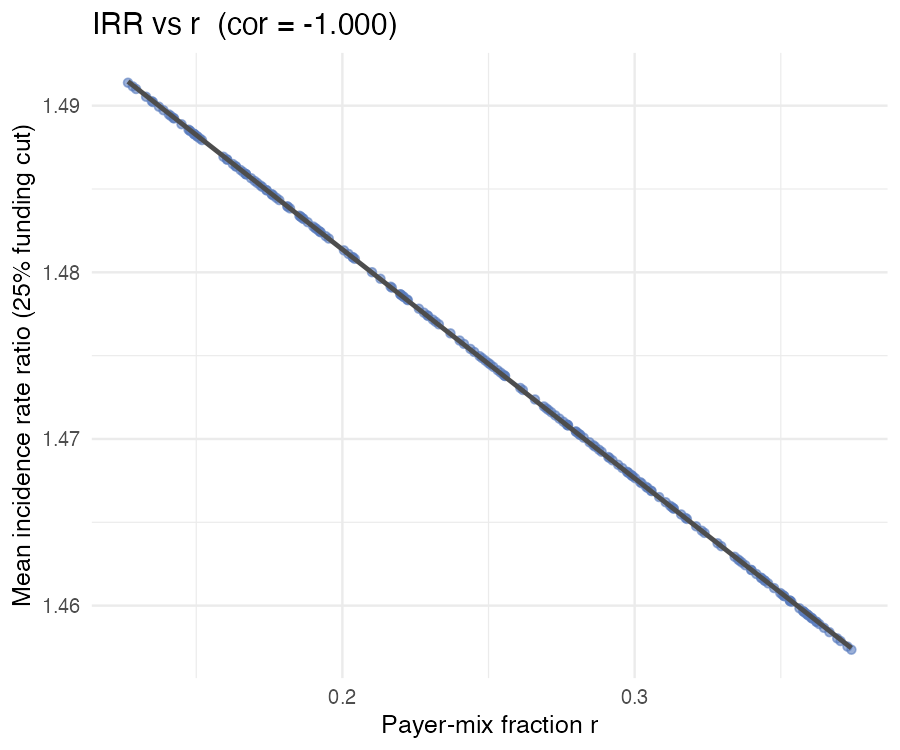
\includegraphics[width=0.48\textwidth]{figures/mc_irr_vs_r.png}
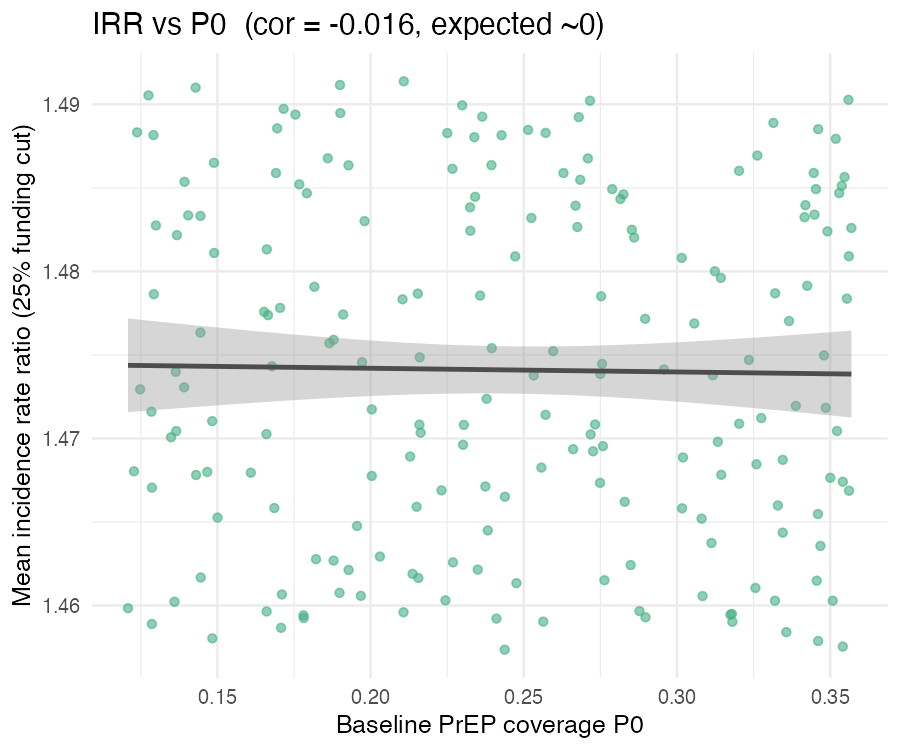
\includegraphics[width=0.48\textwidth]{figures/mc_irr_vs_p0.png}
\caption{Monte Carlo sensitivity ($N=200$ draws): incidence rate ratio at a
25\% funding cut vs.\ $r$ (left, strong negative relationship) and vs.\
$P^0$ (right, no relationship).}
\label{fig:mc-scatter}
\end{figure}

\begin{figure}[htbp]
\centering
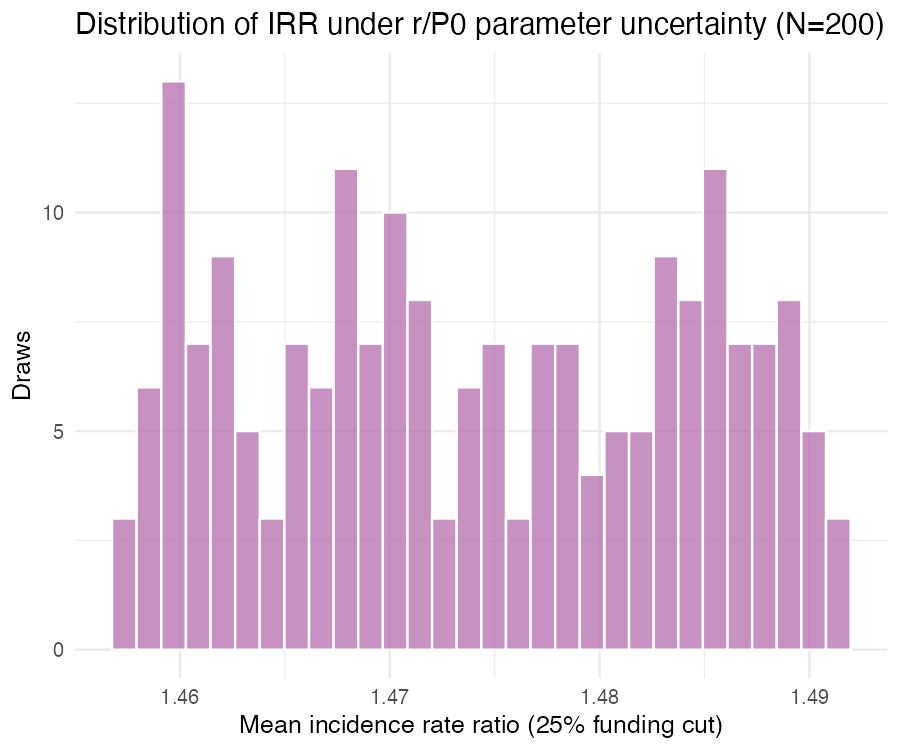
\includegraphics[width=0.55\textwidth]{figures/mc_irr_histogram.png}
\caption{Distribution of the 25\%-funding-cut incidence rate ratio across
the 200 $(r, P^0)$ draws.}
\label{fig:mc-hist}
\end{figure}

\section{Discussion}
\label{sec:discussion}

The revised, population-appropriate payer-mix assumption ($r \approx 25\%$
rather than the national $r=0.78$) produces a materially larger projected
harm from PrEP funding cuts than the paper's currently committed baseline,
consistent with the meeting's hypothesis that the national figure
understates this population's exposure. The effect is robust to a
$\pm 50\%$ uncertainty band on $r$ itself (the sign and rough magnitude of
the shift do not depend on the exact working value chosen within that
range), and --- as anticipated analytically --- entirely insensitive to the
separate, still-open question of the baseline PrEP coverage-level anchor
$P^0$. This means the single highest-value next step from the memo's
action plan (Section~\ref{sec:action}, item 3) is getting AFC's read on a
defensible $r$; refining $P^0$ alone would not change the funding-cut
conclusions.

\subsection{Status}
\label{sec:status}

This is an exploratory sensitivity check, not a revision to the paper. The
committed baseline on \texttt{main} ($r=0.78$) is unchanged. Before the
revised parameter can be adopted in the paper's actual figures (which use
the RAND house style via \texttt{randplot}), we need: (1) AFC's input on a
defensible $r$, and (2) the \texttt{randplot} package, which is not
currently installed anywhere accessible and will be requested from Pedro.
Item~4 of the action plan (mirroring the change into
\texttt{INFORM-HIV-App}) is likewise deferred until $r$ is actually
adopted.

\end{document}
